\documentclass[border=5pt]{standalone}
\usepackage[utf8]{inputenc}
\usepackage[T1]{fontenc}
\usepackage{tikz}
\usetikzlibrary{arrows.meta}
\begin{document}
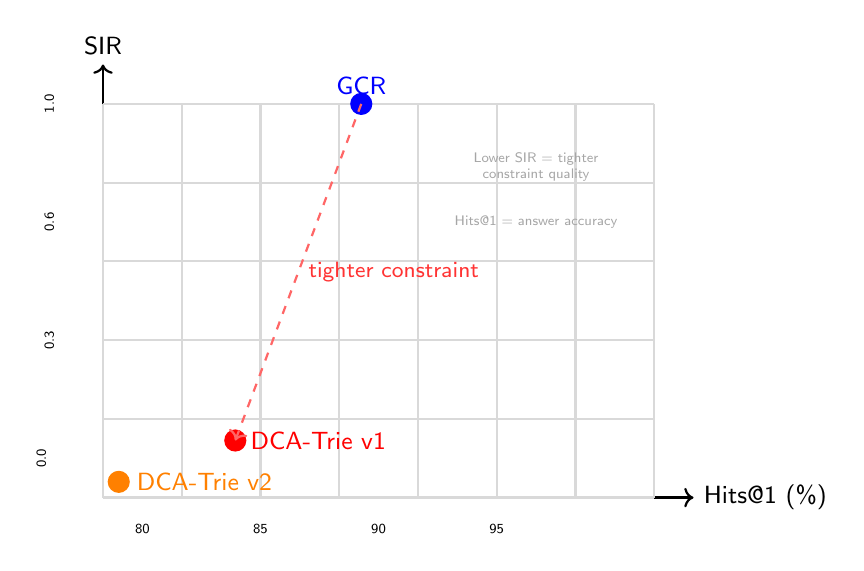
\begin{tikzpicture}[font=\sffamily]
  % Axes
  \draw[->, thick] (0,0) -- (7.5,0) node[right] {\small Hits@1 (\%)};
  \draw[->, thick] (0,0) -- (0,5.5) node[above] {\small SIR};
  \draw[thick, gray!30] (0,0) grid (7,5);

  % Axis labels
  \node[font=\sffamily\tiny] at (0.5, -0.4) {80};
  \node[font=\sffamily\tiny] at (2.0, -0.4) {85};
  \node[font=\sffamily\tiny] at (3.5, -0.4) {90};
  \node[font=\sffamily\tiny] at (5.0, -0.4) {95};
  \node[font=\sffamily\tiny, rotate=90, anchor=south] at (-0.6, 0.5) {0.0};
  \node[font=\sffamily\tiny, rotate=90, anchor=south] at (-0.5, 2.0) {0.3};
  \node[font=\sffamily\tiny, rotate=90, anchor=south] at (-0.5, 3.5) {0.6};
  \node[font=\sffamily\tiny, rotate=90, anchor=south] at (-0.5, 5.0) {1.0};

  % Data points (spread out labels)
  \fill[blue] (3.28, 5.0) circle (4pt) node[above, font=\sffamily\small] {GCR};
  \fill[red] (1.68, 0.725) circle (4pt) node[right, font=\sffamily\small, xshift=2pt]
    {DCA-Trie v1};
  \fill[orange] (0.2, 0.2) circle (4pt) node[right, font=\sffamily\small, xshift=3pt]
    {DCA-Trie v2};

  % Arrow showing the trade-off
  \draw[->, thick, red!60, dashed] (3.28, 5.0) -- (1.68, 0.725)
    node[midway, right, font=\sffamily\footnotesize, text=red!80]
    {tighter constraint};

  % Annotation
  \node[font=\sffamily\tiny, align=center, text=gray!70] at (5.5, 4.2)
    {Lower SIR = tighter\\constraint quality};
  \node[font=\sffamily\tiny, align=center, text=gray!70] at (5.5, 3.5)
    {Hits@1 = answer accuracy};

\end{tikzpicture}
\end{document}
